%\documentclass[]{beamer}
\documentclass[handout]{beamer}
%\usepackage[dvips]{color}
\usepackage{graphicx}
\usepackage{amsmath,amssymb,array,comment,eucal}
\newcommand{\e}{\mathbf{e}}
\renewcommand{\P}{\mathbf{P}}
\newcommand{\F}{\mathbf{F}}
\newcommand{\R}{\textsf{R}}
\newcommand{\mat}[1] {\mathbf{#1}}
%\newcommand{\ind}{\mathrel{\mathop{\sim}\limits^{\mathit{ind}}}}
%\newcommand{\iid}{\mathrel{\mathop{\sim}\limits^{\mathit{iid}}}}
\newcommand{\E}{\textsf{E}}
\newcommand{\SE}{\textsf{SE}}
\newcommand{\SSE}{\textsf{SSE}}
\newcommand{\RSS}{\textsf{RSS}}
\newcommand{\FSS}{\textsf{FSS}}
\renewcommand{\SS}{\textsf{SS}}
\newcommand{\MSE}{\textsf{MSE}}
\newcommand{\SSR}{\textsf{SSR}}
\newcommand{\Be}{\textsf{Beta}}
\newcommand{\St}{\textsf{St}}
%\newcommand{\C}{\textsf{C}}
\newcommand{\GDP}{\textsf{GDP}}
\newcommand{\NcSt}{\textsf{NcSt}}
\newcommand{\Bin}{\textsf{Bin}}
\newcommand{\NB}{\textsf{NegBin}}
\renewcommand{\NG}{\textsf{NG}}
\newcommand{\N}{\textsf{N}}
\newcommand{\Ber}{\textsf{Ber}}
\newcommand{\Poi}{\text{Poi}}
\newcommand{\Gam}{\textsf{Gamma}}
\newcommand{\BB}{\textsf{BB}}
\newcommand{\Gm}{\textsf{G}}
\newcommand{\Un}{\textsf{Unif}}
\newcommand{\Ex}{\textsf{Exp}}
\newcommand{\DE}{\textsf{DE}}
\newcommand{\tr}{\textsf{tr}}
\newcommand{\cF}{{\cal{F}}}
\newcommand{\cL}{{\cal{L}}}
\newcommand{\cI}{{\cal{I}}}
\newcommand{\cB}{{\cal{B}}}
\newcommand{\cP}{{\cal{P}}}
\newcommand{\bbR}{\mathbb{R}}
\newcommand{\bbN}{\mathbb{N}}
\newcommand{\pperp}{\mathrel{{\rlap{$\,\perp$}\perp\,\,}}}
\newcommand{\OFP}{(\Omega,\cF, \P)}
\newcommand{\eps}{\boldsymbol{\epsilon}}
\newcommand{\1}{\mathbf{1}_n}
\newcommand{\gap}{\vspace{8mm}}
\newcommand{\ind}{\mathrel{\mathop{\sim}\limits^{\rm ind}}}
\newcommand{\simiid}{\ensuremath{\mathrel{\mathop{\sim}\limits^{\rm
iid}}}}
\newcommand{\eqindis}{\ensuremath{\mathrel{\mathop{=}\limits^{\rm D}}}}
\newcommand{\iid}{\textit{i.i.d.}}
\newcommand{\SSZ}{S_{zz}}
\newcommand{\SZW}{S_{zw}}
\newcommand{\Var}{\textsf{Var}}
\newcommand{\corr}{\textsf{corr}}
\newcommand{\diag}{\textsf{diag}}
\newcommand{\var}{\textsf{var}}
\newcommand{\Cov}{\textsf{Cov}}
\newcommand{\Sam}{{\cal S}}
\def\H{\mathbf{H}}
\newcommand{\I}{\mathbf{I}}
\newcommand{\Y}{\mathbf{Y}}
\newcommand{\tY}{\tilde{\mathbf{Y}}}
\newcommand{\Yhat}{\hat{\mathbf{Y}}}
\newcommand{\Yobs}{\mathbf{Y}_{{\cal S}}}
\newcommand{\barYobs}{\bar{Y}_{{\cal S}}}
\newcommand{\barYmiss}{\bar{Y}_{{\cal S}^c}}
\def\bv{\mathbf{b}}
\def\X{\mathbf{X}}
\def\tX{\tilde{\mathbf{X}}}
\def\x{\mathbf{x}}
\def\xbar{\bar{\mathbf{x}}}
\def\Xbar{\bar{\mathbf{X}}}
\def\Xg{\mathbf{X}_{\boldsymbol{\gamma}}}
\def\Ybar{\bar{\Y}}
\def\ybar{\bar{y}}
\def\y{\mathbf{y}}
\def\Yf{\mathbf{Y_f}}
\def\W{\mathbf{W}}
\def\L{\mathbf{L}}
\def\w{\mathbf{w}}
\def\U{\mathbf{U}}
\def\V{\mathbf{V}}
\def\Q{\mathbf{Q}}
\def\Z{\mathbf{Z}}
\def\z{\mathbf{z}}
\def\v{\mathbf{v}}
\def\u{\mathbf{u}}

\def\zero{\mathbf{0}}
\def\one{\mathbf{1}}
\newcommand{\taub}{\boldsymbol{\tau}}
\newcommand{\betav}{\boldsymbol{\beta}}
\newcommand{\alphav}{\boldsymbol{\alpha}}
\newcommand{\A}{\mathbf{A}}
\def\a{\mathbf{a}}
\def\K{\mathbf{K}}
\newcommand{\B}{\mathbf{B}}
\def\b{\boldsymbol{\beta}}
\def\bhat{\hat{\boldsymbol{\beta}}}
\def\btilde{\tilde{\boldsymbol{\beta}}}
\def\tb{\tilde{\boldsymbol{\beta}}}
\def\bg{\boldsymbol{\beta_\gamma}}
\def\bgnot{\boldsymbol{\beta_{(-\gamma)}}}
\def\mub{\boldsymbol{\mu}}
\def\tmub{\tilde{\boldsymbol{\mu}}}
\def\muhat{\hat{\boldsymbol{\mu}}}
\def\t{\boldsymbol{\theta}}
\def\tk{\boldsymbol{\theta}_k}
\def\tj{\boldsymbol{\theta}_j}
\def\Mk{\boldsymbol{{\cal M}}_k}
\def\M{\boldsymbol{{\cal M}}}
\def\Mj{\boldsymbol{{\cal M}}_j}
\def\Mi{\boldsymbol{{\cal M}}_i}
\def\Mg{{\boldsymbol{{\cal M}_\gamma}}}
\def\Mnull{\boldsymbol{{\cal M}}_{N}}
\def\gMPM{\boldsymbol{\gamma}_{\text{MPM}}}
\def\gHPM{\boldsymbol{\gamma}_{\text{HPM}}}
\def\Mfull{\boldsymbol{{\cal M}}_{F}}
\def\tg{\boldsymbol{\theta}_{\boldsymbol{\gamma}}}
\def\g{\boldsymbol{\gamma}}
\def\eg{\boldsymbol{\eta}_{\boldsymbol{\gamma}}}
\def\G{\mathbf{G}}
\def\cM{\cal M}
\def\D{\Delta}
\def \shat{{\hat{\sigma}}^2}
\def\uv{\mathbf{u}}
\def\l {\lambda}
\def\d{\delta}
\def\Sigmab{\boldsymbol{\Sigma}}
\def\Lambdab{\boldsymbol{\Lambda}}
\def\lambdab{\boldsymbol{\lambda}}
\def\Mg{{\cal M}_\gamma}
\def\S{{\cal{S}}}
\def\qg{p_{\boldsymbol{\gamma}}}
\def\pg{p_{\boldsymbol{\gamma}}}
\def\t{\boldsymbol{\theta}}  
\def\T{\boldsymbol{\Theta}}  
\usepackage{verbatim}

\usetheme{Warsaw}
\usecolortheme{orchid}
\title{Bayesian Estimation in Linear Models}
\institute{Merlise Clyde}
\author{STA721 Linear Models Duke University}
\date{September 15, 2015}
\logo{duke.eps}

\begin{document}
\maketitle

\begin{frame}
  \frametitle{Bayesian Estimation}
  Model $\Y = \X \b + \eps$  with $\eps \sim \N(\zero_n , \sigma^2
  \I_n)$ \pause
is equivalent to 
$$
\Y \sim \N(\X \b, \I_n/\phi)
$$
\pause
 $\phi = 1/\sigma^2$ is the {\it precision}.   
\pause

\vspace{14pt}
In the  Bayesian paradigm describe uncertainty about unknown
parameters using probability distributions
\pause
\begin{itemize}
\item  Prior Distribution $p(\b, \phi)$ describes uncertainty about
  parameters prior to seeing the data \pause
\item Posterior Distribution $p(\b, \phi \mid \Y)$ describes
  uncertainty about the parameters after updating  believes given the
  observed data \pause
\item updating rule is based on Bayes Theorem
$$p(\b, \phi \mid \Y) \propto \cL(\b, \phi) p(\b, \phi)$$
\pause
\end{itemize}
 reweight prior beliefs by likelihood of parameters  under observed data
\end{frame}

\begin{frame}
  \frametitle{Posterior}
  Posterior is obtained by conditional distribution theory \pause

  Let $\t = (\b, \phi)^T$ \pause
\begin{eqnarray*}
  p(\t \mid \Y ) & = & \frac{p(\Y \mid \t) p(\t) }
{ \int_{\T} p(\Y \mid \t)   p(\t) \, d\t} \pause \\
& = &  \frac{p(\Y, \t)}{p(\Y)}
\end{eqnarray*}
\pause
$p(\Y)$, the normalizing constant, is the marginal distribution of the data.
\pause
\vfill

Easiest to work with Bayes Theorem in proportional form and then
identify the normalizing constant.
\end{frame}

\begin{frame}
  \frametitle{Prior Distributions}
Factor joint prior distribution  $$p(\b, \phi) = p(\b \mid \phi) p(\phi)$$
\pause

Convenient choice is to take \pause
\begin{itemize}
\item $\b \mid \phi \sim \N(b_0, \Phi_0^{-1}/\phi)$ where $b_0$ is the prior
  mean and $\Phi^{-1}/\phi$ is the prior covariance of $\b$ \pause
\item $\phi \sim \G( \nu_0/2, \SS_0/2)$  with $\E(\sigma^2) =
  \SS_0/(\nu_0 - 2)$ \pause
$$p(\phi) = \frac{1}{\Gamma{(\nu_0/2)}} 
\left(\frac{\SS_0}{2} \right)^{\nu_0/2} 
\phi^{\nu_0/2 - 1}
 e^{- \phi \SS_0/2}
 $$\pause
\item $(\b, \phi)^T \sim \NG(\bv_0, \Phi_0, \nu_0, \SS_0)$ \pause
\item Conjugate  ``Normal-Gamma'' family implies \pause
$$(\b, \phi)^T \mid \Y \sim \NG(\bv_n, \Phi_n, \nu_n, \SS_n)$$
\end{itemize}
\end{frame}


\begin{frame}
\frametitle{Finding the Posterior Distribution}
Express Likelihood: $\cL(\beta, \phi) \propto \phi^{n/2} e^{- \phi \frac{\SSE}{2}}
e^{-\frac{\phi}{2} (\b - \bhat)^T(\X^T\X) (\b - \bhat)}$ \pause
\begin{eqnarray*}
 p(\b, \phi \mid \Y) &\propto&  \phi^{\frac {n + p + \nu_0}{ 2} - 1}
 e^{- \frac \phi 2 ( \SSE + \SS_0) } \\
 & & e^{-\frac{\phi}{2} (\b - \bhat)^T(\X^T\X) (\b - \bhat)}
 e^{- \frac{\phi}{2} (\b - \bv_0)^T \Phi (\b - \bv_0) }  
\end{eqnarray*} \pause

Quadratic in Normal
$$\exp\left\{- \frac{\phi}{2} (\b - \bv)^T \Phi (\b - \bv) \right\} = \exp\left\{-
  \frac{\phi}{2} (\b^T \Phi \b - 2 \b^T \Phi \bv + \bv^T\Phi \bv )\right\}$$
\pause

  \begin{itemize}
  \item Expand quadratics and regroup terms \pause 
  \item Read off posterior precision from Quadratic in $\b$ \pause 
  \item Read off posterior mean from Linear term in $\b$ \pause 
  \item will need to complete the quadratic in the posterior mean
  \end{itemize}
\end{frame}
\begin{frame}
  \frametitle{ Expand and Regroup}
  Quadratic in Normal
$$\exp\left\{- \frac{\phi}{2} (\b - \bv)^T \Phi (\b - \bv) \right\} = \exp\left\{-
  \frac{\phi}{2} (\b^T \Phi \b - 2 \b^T \Phi \bv + \bv^T\Phi \bv )\right\}$$
\pause 

\begin{eqnarray*}
 p(\b, \phi \mid \Y) &\propto&  \phi^{\frac {n + p + \nu_0}{ 2} - 1}
 e^{- \frac \phi 2 ( \SSE + \SS_0) }  \\
 & & e^{-\frac{\phi}{2} (\b - \bhat)^T(\X^T\X) (\b - \bhat)}
 e^{- \frac{\phi}{2} (\b - \bv_0)^T \Phi_0 (\b - \bv_0) } \pause  \\ 
 & = & \phi^{\frac {n + p + \nu_0}{ 2} - 1}
 e^{- \frac \phi 2 ( \SSE + \SS_0) } \pause \\
& &  e^{ -\frac{\phi}{2} \left(  \b^T (\X^T\X + \Phi_0) \b  \right) } \pause \\
& &  e^{  -\frac{\phi}{2} \left( -2 \b^T (\X^T\X \bhat  + \Phi_0 \bv_0)
   \right)} \pause \\
& &  e^{  -\frac{\phi}{2} (\bhat^T \X^T\X \bhat + \bv_0^T \Phi_0 \bv_0
  )}
\end{eqnarray*}




\end{frame}
\begin{frame}
  \frametitle{ Identify Hyperparameters and Complete the Quadratic}
  Quadratic in Normal
$$\exp\left\{- \frac{\phi}{2} (\b - \bv)^T \Phi (\b - \bv) \right\} = \exp\left\{-
  \frac{\phi}{2} (\b^T \Phi \b - 2 \b^T \Phi \bv + \bv^T\Phi \bv )\right\}$$
\pause 


Let $\Phi_n = \X^T\X + \Phi_0$ \pause
  \begin{eqnarray*}
 p(\b, \phi \mid \Y) &\propto&  \phi^{\frac {n + p + \nu_0}{ 2} - 1}
 e^{- \frac \phi 2 ( \SSE + \SS_0) } \pause \\
& &  e^{ -\frac{\phi}{2} \left(  \b^T \alert<4>{(\X^T\X + \Phi_0)} \b
  \right) } \pause\\
& &  e^{  -\frac{\phi}{2} \left( -2 \b^T \alert<5>{\Phi_n \Phi_n^{-1}} (\X^T\X \bhat  + \Phi_0 \bv_0)
   \right)} \pause\\
& &  e^{ -\frac{\phi}{2} (\alert<6>{\bv_ n^T \Phi_n \bv_n - \bv_n^T \Phi_0
  \bv_n}) } \pause \\
& &  e^{  -\frac{\phi}{2} (\bhat^T \X^T\X \bhat + \bv_0^T \Phi_0 \bv_0
  )} \pause \\
& = &
  \phi^{\frac {n + p+  \nu_0}{ 2} - 1}
 e^{- \frac \phi 2 ( \SSE + \SS_0  + \bhat^T \X^T\X \bhat + \bv_0^T \Phi_0 \bv_0
 - \bv_n^T \Phi_n \bv_n)}  \pause  \\
& &  e^{ -\frac{\phi}{2} \left(  \b^T \alert{(\Phi_n)} \b
  \right) } \pause\\
& &  e^{  -\frac{\phi}{2} \left( -2 \b^T \Phi_n\alert{\Phi_n^{-1} (\X^T\X \bhat  + \Phi_0 \bv_0)}
   \right)} \pause\\
& &  e^{ -\frac{\phi}{2} (\alert{\bv_ n^T \Phi_n \bv_n}) } 
  \end{eqnarray*}

\end{frame}
\begin{frame}
  \frametitle{Posterior Distribution}
  \begin{eqnarray*}
 p(\b, \phi \mid \Y) &\propto&
  \phi^{\frac {n +  \nu_0}{ 2} - 1}
 e^{- \frac \phi 2 ( \SSE + \SS_0  + \bhat^T \X^T\X \bhat + \bv_0^T \Phi_0 \bv_0
 - \bv_n^T \Phi_n \bv_n)} \\
& & \phi^{\frac p 2} e^{- \frac{\phi}{2} (\b - \bv_n)^T \Phi_n (\b -
  \bv_n) }  \pause  \\
& & \\
\Phi_n & = & \X^T\X +  \Phi_0 \pause \\
\bv_n &  = & \Phi_n^{-1} (\X^T\X \bhat  + \Phi_0 \bv_0) \pause
  \end{eqnarray*}

Posterior Distribution
  \begin{eqnarray*}
\b \mid \phi, \Y & \sim &\N(\bv_n, (\phi \Phi_n)^{-1}) \pause \\
\phi \mid \Y &\sim &\G(\frac{n + \nu_0}{2}, \frac{\SSE + \SS_0 + \bhat^T \X^T\X \bhat + \bv_0^T \Phi_0 \bv_0
 - \bv_n^T \Phi_n \bv_n}{2})
  \end{eqnarray*}
  

\end{frame}
\begin{frame}
  \frametitle{Marginal Distribution from Normal--Gamma }
  \begin{theorem}
    Let  $\t \mid \phi \sim \N(m, \frac{1}{\phi} \Sigma)$ and $\phi \sim
    \G(\nu/2, \nu \shat/2)$. Then  $\t$ ($p \times 1)$ has a $p$
    dimensional multivariate $t$ distribution $$\t \sim t_\nu( m,
    \shat \Sigma )$$ with density
$$p(\t) \propto  \left[ 1 + \frac{1}{\nu}  \frac{ (\t - m)^T
    \Sigma^{-1} (\t - m)}{\shat} \right]^{- \frac{p + \nu}{2}}$$
  \end{theorem}
\end{frame}

\begin{frame}
  \frametitle{Derivation}
Marginal density  $p(\t) = \int p(\t \mid \phi) p(\phi) \, d\phi$
\pause
\begin{eqnarray*}
  p(\t) & \propto & \int |\Sigma/\phi|^{-1/2} 
e^{- \frac{\phi}{2} (\t - m)^T
    \Sigma^{-1} (\t - m)}  \phi^{\nu/2 - 1} e^{- \phi \frac{\nu
      \shat}{2}}\, d \phi \pause \\
  & \propto & \int \phi^{p/2} \phi^{\nu/2 - 1}
e^{- \phi \frac{(\t - m)^T
    \Sigma^{-1} (\t - m)+  \nu
      \shat}{2}}\, d \phi \pause \\
 & \propto & \int \phi^{\frac{p +\nu}{2} - 1}
e^{- \phi \frac{(\t - m)^T
    \Sigma^{-1} (\t - m)+  \nu
      \shat}{2}} \, d \phi \pause \\
& = & \Gamma((p + \nu)/2 ) \left( \frac{(\t - m)^T
    \Sigma^{-1} (\t - m)+  \nu
      \shat}{2} \right)^{- \frac{p + \nu}{2}} \pause \\
& \propto &  \left( (\t - m)^T
    \Sigma^{-1} (\t - m)+  \nu
      \shat \right)^{- \frac{p + \nu}{2}} \pause \\
& \propto &  \left( 1 + \frac{1}{\nu}  \frac{(\t - m)^T
    \Sigma^{-1} (\t - m)}{\shat}
       \right)^{- \frac{p + \nu}{2}}
\end{eqnarray*}
\end{frame}

\begin{frame}
  \frametitle{Marginal Posterior Distribution of $\b$}
  \begin{eqnarray*}
\b \mid \phi, \Y  & \sim & \N( \bv_n, \phi^{-1} \Phi_n^{-1}) \pause \\    
 \phi \mid \Y & \sim & \G\left(\frac{\nu_n}{2},  \frac{\SS_n}{ 2} \right) 
  \end{eqnarray*}
\pause

Let $\shat = \SS_n/\nu_n$  (Bayesian MSE) \pause

Then the marginal posterior distribution of $\b$ is 
$$
\b  \mid \Y \sim t_{\nu_n} (\bv_n, \shat \Phi_n^{-1})
$$ \pause


Any linear combination $\lambda^T\b$
$$\lambda^T\b  \mid \Y \sim t_{\nu_n}
(\lambda^T\bv_n, \shat \lambda^T\Phi_n^{-1}\lambda)$$ has a univariate
$t$ distribution with $\v_n$ degrees of freedom

\end{frame}

\begin{frame}
  \frametitle{Predictive Distribution}
Suppose $\Y^* \mid \b, \phi \sim \N(\X^* \b , \I/\phi)$  and is conditionally
independent of $\Y$ given $\b$ and $\phi$ \pause
\vspace{18pt}

What is the predictive distribution of $\Y^* \mid \Y$? \pause

\vspace{18pt}
$\Y^* = \X^* \b + \eps^*$ and $\eps^*$ is independent of $\Y$ given
$\phi$ \pause

\begin{eqnarray*}
\X^* \b + \eps^* \mid \phi, \Y & \sim & \N(\X^*\bv_n, (\X^{*} \Phi_n^{-1} \X^{*T}
+ \I)/\phi)  \pause \\
\Y^* \mid \phi, \Y & \sim & \N(\X^*\bv_n, (\X^{*} \Phi_n^{-1} \X^{*T}
+ \I)/\phi)  \pause \\
\phi \mid \Y & \sim & \G\left(\frac{\nu_n}{2},
  \frac{\shat \nu_n}{ 2} \right)  \pause \\
\Y^* \mid \Y & \sim & t_{\nu_n}( \X^*\bv_n, \shat (\I + \X^* \Phi_n^{-1} \X^T))
\end{eqnarray*}
\end{frame}
\begin{frame}
  \frametitle{Alternative Derivation}
Conditional Distribution:
\begin{eqnarray*}
f(\Y^* \mid \Y) & = & \frac{f(\Y^*, \Y)}{f(\Y)} \pause \\
 & = & \frac{
\iint f(\Y^*, \Y \mid \b, \phi) p(\b, \phi) d\b\, d\phi
}
{
  f(\Y)
}  \pause \\
 & = & \frac{
\iint f(\Y^*\mid \b, \phi) f(\Y \mid \b, \phi) p(\b, \phi) d\b\, d\phi
}
{
  f(\Y)
}  \pause \\
 & = & 
\iint f(\Y^*\mid \b, \phi)  p(\b, \phi \mid \Y) d\b\, d\phi \pause
\end{eqnarray*}
$$\Y^* = \X^* \b + \eps^* \mid \Y, \phi \sim \N(\X^* \bv_n, \phi^{-1}(\I +
\X^* \Phi_n \X^{*T}))$$ \pause
Use result about Marginals of Normal-Gamma family to integrate out $\phi$ 
\end{frame}

\begin{frame}
  \frametitle{Conjugate Priors}
  \begin{definition}
    A class of prior distributions $\cP$ for $\t$ is conjugate for a
    sampling model $p(y \mid \t)$ if for every $p(\t) \in \cP$, $p(\t
    \mid \Y) \in \cP$.
  \end{definition}
\pause  
  Advantages: \pause
  \begin{itemize}
  \item Closed form distributions for most quantities; bypass MCMC for
    calculations \pause
  \item Simple updating in terms of sufficient statistics ``weighted
    average'' \pause
  \item Interpretation as prior samples - prior sample size \pause
  \item Elicitation of prior through imaginary or historical data \pause
  \item limiting ``non-proper'' form recovers MLEs \pause
  \end{itemize}
Choice of conjugate prior?
\end{frame}

\begin{frame}
  \frametitle{Unit Information Prior}

Unit information prior $\b \mid \phi \sim \N(\bhat, n
   (\X^T\X)^{-1}/\phi)$ \pause
  \begin{itemize}
\item Fisher Information is $\phi \X^T\X$ based on a sample of $n$
  observations \pause
\item Inverse Fisher information is covariance matrix of MLE \pause
\item ``average information'' in one observation is  $\phi \X^T\X /n$ \pause
\item center prior at MLE and base covariance on the information in
  ``1'' observation \pause
\item  Posterior mean 
$$\frac{n}{1 + n} \bhat +  \frac{1}{1 + n}\bhat = \bhat$$ \pause
\item Posterior Distribution 
$$\b \mid \Y, \phi \sim \N\left( \bhat, \frac{n}{1 + n} (\X^T\X)^{-1}
  \phi^{-1} \right)$$ \pause
    \end{itemize}
Cannot represent real prior beliefs; double use of data
\end{frame}

\begin{frame}
  \frametitle{Zellner's $g$-prior}
Zellner's g-prior(s) $\b \mid \phi \sim \N(\bv_0, g
    (\X^T\X)^{-1}/\phi)$ \pause

$$\b \mid \Y, \phi \sim \N\left( \frac{g}{1 + g} \bhat +  \frac{1}{1 + g}
\bv_0, \frac{g}{1 + g} (\X^T\X)^{-1} \phi^{-1} \right)$$ \pause

\begin{itemize}
\item Invariance: Require posterior of   $\X \b$  equal the posterior of $\X \H \alphav$
\pause   ($\a_0 = \H^{-1} \bv_0$)  ( take $\bv_0 = \zero$)

\item Choice of $g$?  \pause
\item $\frac{g}{1 + g}$  weight given to the data \pause
\item Fixed $g$ effect does not vanish as $n \to \infty$ 
\item Use $g = n$ or place a prior diistribution on $g$
\end{itemize}


\end{frame}
\begin{frame}
  \frametitle{Shrinkage}
 Posterior mean under  $g$-prior  with $\bv_0 = 0$
$\frac{g}{1 +g} \bhat $

\centerline{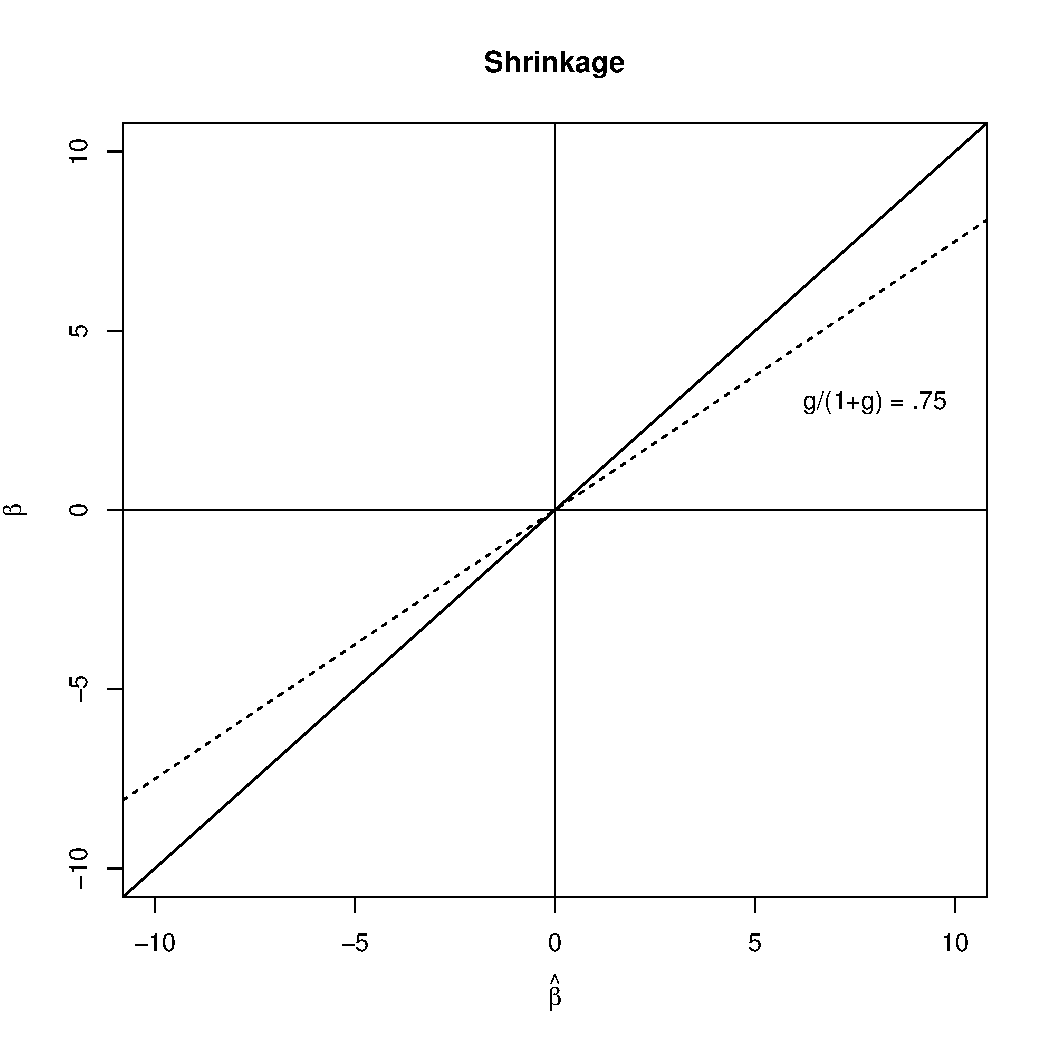
\includegraphics[height=3in]{shrinkage}}
\end{frame}

\end{document}

\begin{frame}
  \frametitle{Jeffreys Prior}
  
Jeffreys proposed a default  procedure so that resulting prior
would be invariant to model parameterization  \pause

$$p(\t) \propto |\cI(\t)|^{1/2}$$
\pause
where $\cI(\t)$ is the  Expected Fisher Information matrix
\pause
$$
\cI(\theta) = - \E[ \left[ \frac{\partial^2 \log(\cL(\t))}{\partial
  \theta_i \partial \theta_j} \right] ]
$$
\end{frame}
\begin{frame}
  \frametitle{Fisher Information Matrix}
Log Likelihood
$$
    \log(\cL(\b, \phi))  =  \, \frac{n}{2} \log(\phi)  - \frac{\phi}{2}
     \| (\I - \P_\x) \Y\|^2  
 - \frac{\phi}{2}(\b - \bhat)^T(\X^T\X)(\b - \bhat) 
$$ \pause
  \begin{eqnarray*}
\frac{\partial^2 \log \cL} { \partial \t \partial \t^T} & = &
\left[
  \begin{array}{cc}
    -\phi (\X^T\X) & -(\X^T\X) (\b - \bhat) \\
  - (\b - \bhat)^T (\X^T\X) & -\frac{n}{2} \frac{1}{\phi^2} \\
  \end{array}
\right] \pause \\
\E[\frac{\partial^2 \log \cL} { \partial \t \partial \t^T}] & = &
\left[
  \begin{array}{cc}
    -\phi (\X^T\X) & \zero_p \\
  \zero_p^T & -\frac{n}{2} \frac{1}{\phi^2} \\
  \end{array}
\right] \pause \\
& & \\
\cI((\b, \phi)^T) & = & \left[
  \begin{array}{cc}
    \phi (\X^T\X) & \zero_p \\
  \zero_p^T & \frac{n}{2} \frac{1}{\phi^2} 
  \end{array}
\right]
  \end{eqnarray*}
\end{frame}
\begin{frame}
  \frametitle{Jeffreys Prior}
  Jeffreys Prior 
  \begin{eqnarray*}
  p_J(\b, \phi)  & \propto & |\cI((\b, \phi)^T) |^{1/2}   \pause \\
               & = & |\phi (\X^T\X|^{1/2} \left(\frac{n}{2}
                 \frac{1}{\phi^2} \right)^{1/2} \pause \\
  & \propto  &  \phi^{p/2 - 1} |\X^T\X|^{1/2} \pause \\
  & \propto & \phi^{p/2 - 1}  \pause
  \end{eqnarray*}
  Improper prior   $\iint p_J(\b, \phi) \, d\b \, d\phi $ not finite
  
\end{frame}
\begin{frame}
  \frametitle{Formal Bayes Posterior}
$$  p(\b, \phi \mid \Y) \propto p(\Y \mid \b, \phi)  \phi^{p/2 - 1} $$
\pause
if this is integrable, then renormalize to obtain formal posterior
distribution \pause


\begin{eqnarray*}
  \b \mid \phi, \Y & \sim & \N(\bhat, (\X^T\X)^{-1} \phi^{-1}) \\
  \phi \mid \Y & \sim& \G(n/2, \| \Y - \X\bhat \|^2/2)
\end{eqnarray*} \pause
Limiting case of Conjugate prior with $\bv_0 = 0$, $\Phi = \zero$,
$\nu_0 = 0$ and $\SS_0 = 0$ \pause

Posterior does not depend on dimension $p$;   \pause

\vfill
Jeffreys did not recommend using this 
\end{frame}
\begin{frame}
  \frametitle{Independent Jeffreys Prior}
  \begin{itemize}
  \item  Treat $\b$ and $\phi$ separately  (``orthogonal
    parameterization'') \pause
  \item $p_{IJ}(\b) \propto |\cI(\b)|^{1/2}$ \pause
\item $p_{IJ}(\phi) \propto |\cI(\phi)\|^{1/2}$ \pause
  \end{itemize}
$$
\cI((\b, \phi)^T)  =  \left[
  \begin{array}{cc}
    \phi (\X^T\X) & \zero_p \\
  \zero_p^T & \frac{n}{2} \frac{1}{\phi^2} 
  \end{array}
\right]
$$
\pause
$$p_{IJ}(\b) \propto |\phi \X^T\X|^{1/2} \propto 1$$ \pause
$$p_{IJ}(\phi) \propto \phi^{-1}$$ \pause

Independent Jeffreys Prior is 
$$p_{IJ}(\beta, \phi) \propto p_{IJ}(\b) p_{IJ}(\phi) = \phi^{-1}$$
  
\end{frame}
\begin{frame}
  \frametitle{Formal Posterior Distribution}
  With Independent Jeffreys Prior
$$p_{IJ}(\beta, \phi) \propto p_{IJ}(\b) p_{IJ}(\phi) = \phi^{-1}$$
\pause
Formal Posterior Distribution
\pause
\begin{eqnarray*}
  \b \mid \phi, \Y & \sim & \N(\bhat, (\X^T\X)^{-1} \phi^{-1}) \pause \\
  \phi \mid \Y & \sim& \G((n-p)/2, \| \Y - \X\bhat \|^2/2) \pause\\
\b \mid \Y & \sim & t_{n-p}(\bhat, \shat (\X^T\X)^{-1})\pause
\end{eqnarray*}
Bayesian Credible Sets
$p(\b \in C_\alpha) = 1- \alpha$ correspond to frequentist Confidence
Regions

$$\frac{\lambdab^T\b - \lambdab\bhat}
{\sqrt{\shat \lambdab^T(\X^T\X)^{-1} \lambdab}} \sim t_{n-p}$$

\end{frame}
\begin{frame}
  \frametitle{Disadvantages of Conjugate Priors}
  Disadvantages: \pause
\begin{itemize}
\item Results  may have be sensitive to prior ``outliers'' due to
  linear updating \pause
\vspace{1.5in}

\item Cannot capture all possible prior beliefs \pause
\item Mixtures of Conjugate Priors
\end{itemize}
\end{frame}
\end{document}
\begin{frame}
  \frametitle{Mixtures of Conjugate Priors}
  \begin{theorem}[Diaconis \& Ylivisaker 1985]  Given a sampling model
  $p(y \mid \t)$ from an exponential family, any prior distribution
  can be expressed as a mixture of conjugate prior distributions 
 \end{theorem}

 \begin{itemize}
 \item Prior $p(\t) = \int p(\t \mid \omega) p(\omega)\, d \omega$ \pause
 \item Posterior \pause
   \begin{eqnarray*}
   p(\t \mid \Y)  &\propto & \int p(\Y \mid \t) p(\t \mid \omega)
   p(\omega) \, d\omega \pause \\
 & \propto & \int  \frac{  p(\Y \mid \t) p(\t \mid \omega) } {p(\Y \mid
   \omega)}  p(\Y \mid
 \omega) p(\omega ) \, d \omega  \pause \\
& \propto & \int p(\t \mid \Y, \omega)  p(\Y \mid
 \omega) p(\omega ) \, d \omega \pause \\
 p(\t \mid \Y) & =  & \frac{\int p(\t \mid \Y, \omega)  p(\Y \mid
 \omega) p(\omega ) \, d \omega }
{\int p(\Y \mid
 \omega) p(\omega ) \, d \omega }
       \end{eqnarray*}

 \end{itemize}
\end{frame}

\end{document}

